\documentclass[11pt, a4paper]{article} 

\usepackage[utf8]{inputenc}  

\usepackage{caption}    		

\usepackage{color}
\usepackage{etoolbox}    
\usepackage[bottom]{footmisc}  
\usepackage{graphicx}       
\usepackage[hidelinks]{hyperref}		
%\usepackage{listings}
\usepackage{lscape}
\usepackage{euler}     
\usepackage[margin=1in]{geometry}

\usepackage{Sweave}
%\usepackage{C:/Program Files/R/R-3.1.2/share/texmf/tex/latex/Sweave.sty}

\frenchspacing 
%------------------------------------------------------------------------------------------------------
%------------------------------------------------------------------------------------------------------

\begin{document}
\Sconcordance{concordance:sweave_document_TB.tex:sweave_document_TB.Rnw:%
<<<<<<< Updated upstream
1 39 1 1 0 22 1 1 8 4 1 1 7 1 2 9 1 2 2 4 1 1 4 1 1 1 4 20 1}
=======
1 39 1 1 0 24 1 1 7 1 2 6 1 1 4 1 2 3 1}
>>>>>>> Stashed changes


\date{}
\title{Appendix}

\maketitle

%------------------------------------------------------------------------------------------------------
%------------------------------------------------------------------------------------------------------










\bigskip


%The dataset to be working with should be named ``data.sub''. The conducted analysis using the function rma from the metafor pacakge should be renamed as such: rma of a random effects model should be named ``rma.RE'' and an rma of a fixed effects model should be named ``rma.FE'' in order for the automatisation to work. IF a meta-regression has been conducted, it should be called ``rma.RE.meta'' or ``rma.FE.meta'' respectively. Other than that, the metafor package in R needs to be installed.  




The method used in the rma object for the meta-analysis is REML and the measure used is SMD.





%Creates a table for the results of the meta-analysis.Values for ES, SE (ES),pES, CI, I2, Egger value and fail-safe number. 




% latex table generated in R 3.1.2 by xtable 1.7-4 package
% Wed Nov 26 12:18:31 2014
\begin{table}[ht]
\centering
\caption{Results of the meta-analysis. ES = Effect Size, Q = Test for residual heterogeneity, $I^2$ = Residual heterogeneity, Egger's test (SE used as the predictor) and the fails-safe number (FSN) for publication bias testing according to 'Rosenberg'.} 
{\footnotesize
\scalebox{0.9}{
\begin{tabular}{rccccccccccc}
  \hline
 & {ES} & \parbox{1cm}{SE of ES} & CI (lb) & CI (ub) & P(ES) & Q & P(Q) & $I^2$ & Egger & P(Egger) & FSN \\ 
  \hline
Meta-Analysis & -0.28 & 0.12 & -0.52 & -0.04 & 0.02 & 47.05 & 0.12 & 27.22 & -0.44 & 0.66 & 68.00 \\ 
   \hline
\end{tabular}
}
}
\end{table}

%Rosenberg method used as its consistent with how mean effect sizes are calculated. FSN assumes that the mean effect size of missing studies is that predicted by the null hypothesis. This will inflate N if there is, in fact, a publication bias agains results in the opposite direction to the current mean effect. 

{The fail-safe number suggests that the meta-analysis is not robust against publication bias.} This is done by checking if the fail-safe number is greater than (5*(number of studies) +5). 



\noindent
The Eggers test for testing funnel plot asymmetry suggests that there is no publication bias because there is no relationship between the effect size and the sample size. The funnel plot is symmetrical

%Eggers test, the slope will indicate the size and direction of the effect size and the intercept will be 0. The deviation of the intercept from zero provides and index of degree of asymmetry.Tests for a relationship between observed outcomes and sei. If a relationship is present, implies asymmetry. In our case, pval not significant, so no asymmetry--> no publication bias. 


%Creates a forest plot of the meta-analysis.


\begin{figure}[!h]
\captionsetup{width=0.6\textwidth}
\centering
\includegraphics[width=0.7\textwidth]{sweave_document_TB-forest}
\caption{Forest plot of a random effects model. The study and its respectice effect size (ES) [+- 95\% CI] are shown. The weight given to the study (\%) (the inverse to the study variance) is depicted as well.}
\label{fig:forestplot}
\end{figure}

If the effect sizes in the forest plot vary too  much, then heterogeneity should be explored in more depth. This is done by taking \emph{explanatory variabales} into account in a meta-regression. When taking various explanatory variables (moderators) into account, the resulting forest plot shows the way in which the effect size varies when looking at the particular moderator. 


\bigskip
\bigskip

%Table of the meta-regression, in this case with various moderators. 


% latex table generated in R 3.1.2 by xtable 1.7-4 package
% Wed Nov 26 12:18:31 2014
\begin{table}[ht]
\centering
\caption{Results of the meta-regression (mixed-effects model). The model results are shown taking a moderator or various moderators into account and displaying their coefficients. Results for the whole model are displayed as Q = Test for residual heterogeneity, $I^2$ = residual heterogeneity and QM = Test of Moderators.} 
{\footnotesize
\scalebox{0.9}{
\begin{tabular}{rccccc|ccccc}
  \hline
 & {ES} & \parbox{1cm}{SE of ES} & CI (lb) & CI (ub) & P(ES) & Q & P(Q) & I^2 & QM & P(QM) \\ 
  \hline
intrcpt & -0.353 & 0.766 & -1.85 & 1.15 & 0.645 & 22.7 & 0.54 & 0.000493 & 24.4 & 0.0278 \\ 
  continentAS & -0.377 & 0.423 & -1.21 & 0.452 & 0.373 &  &  &  &  &  \\ 
  continentCA & -0.0485 & 0.61 & -1.24 & 1.15 & 0.937 &  &  &  &  &  \\ 
  continentSA & -0.627 & 0.375 & -1.36 & 0.108 & 0.0945 &  &  &  &  &  \\ 
  metricric & 0.119 & 0.254 & -0.38 & 0.617 & 0.641 &  &  &  &  &  \\ 
  disturbanceagf & 0.331 & 0.745 & -1.13 & 1.79 & 0.657 &  &  &  &  &  \\ 
  disturbanceagr & 0.701 & 0.936 & -1.13 & 2.54 & 0.454 &  &  &  &  &  \\ 
  disturbancebur & 0.723 & 0.731 & -0.709 & 2.15 & 0.322 &  &  &  &  &  \\ 
  disturbanceoth & 0.728 & 0.903 & -1.04 &  2.5 & 0.42 &  &  &  &  &  \\ 
  disturbancepas & -0.0589 & 0.979 & -1.98 & 1.86 & 0.952 &  &  &  &  &  \\ 
  disturbancepla & -0.203 & 0.868 & -1.9 &  1.5 & 0.815 &  &  &  &  &  \\ 
  disturbancesec & 0.399 & 0.723 & -1.02 & 1.82 & 0.581 &  &  &  &  &  \\ 
  disturbancesel & 0.796 & 0.691 & -0.559 & 2.15 & 0.25 &  &  &  &  &  \\ 
  disturbanceshd & -0.908 & 0.783 & -2.44 & 0.626 & 0.246 &  &  &  &  &  \\ 
   \hline
\end{tabular}
}
}
\end{table}\bigskip

%Forest plot of the meta-regression model

\begin{figure}[h!]
\captionsetup{width=0.6\textwidth}
\centering
\includegraphics[width=0.65\textwidth]{sweave_document_TB-forestreg}
\caption{Forest plot of a random effects meta regression model. The study and its respectice effect size (ES) [+- 95\% CI] are shown. The weight given to the study (\%) (the inverse to the study variance) is depicted as well.}
\label{fig:forestplotreg}
\end{figure}



%Funnelplot of meta-analysis to assess publication bias. 

\begin{figure} [h!]
\captionsetup{width=0.6\textwidth}
\centering
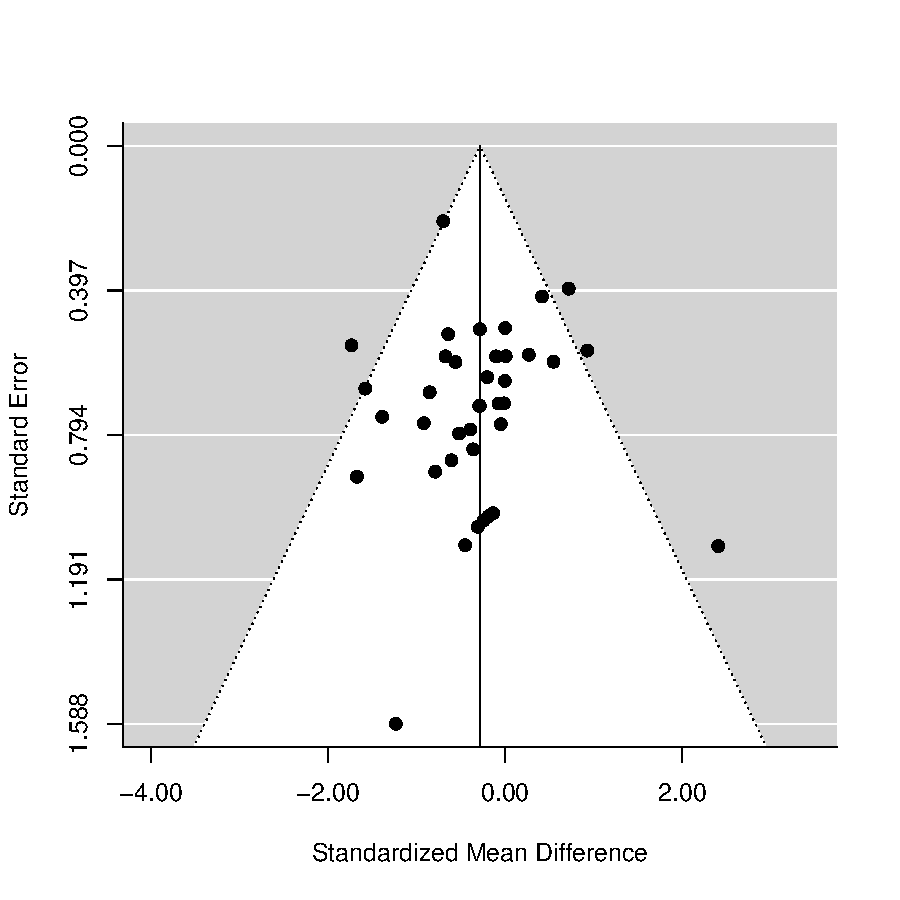
\includegraphics[width=0.7\textwidth]{sweave_document_TB-funnelplot}
\caption{Funnel plot of a random effects model displaying possible publication bias. The true ES is displayed by the solid verical line.}
\end{figure}

To assess possible publication bias, funnel plots can be used for visualization purposes.When publication bias is absent, the plot should have a symmetrical shape of a funnel around the mean effect size. This is because the precision of the estimation of effect size should increase with sample size (smaller standard error). If many studies lie outside of this funnel shaped space, then the studies used might need to be reviewed and checked for...  
\bigskip

%Plot of the diagnostics

\begin{figure} [h!]
\captionsetup{width=0.6\textwidth}
\centering
\includegraphics[width=0.9\textwidth]{sweave_document_TB-diagnostics}
\caption{Diagnostic plots for diagnostics of meta analysis. Standardized residual plot, normal Q-Q plot, Baujat heterogeneity plot and Galbrath's radial plot are shown.}
\label{fig:diagnostics}
\end{figure}

The Baujat plot detects sources of heterogeneity. Studies which are aggregated to the far left of the plot contribute to more heterogeneity in the analysis. Plots which have a high contribution to the overall heterogeneity and have a high influence on the overall result, should be looked at more critically. These studies should be compared to the results obtained in the sensitivity analysis table~\ref{xtable3}.  


The Galbraith plot provides visual information on the heterogeneity of the meta-analysis. Values which are closer to the origin have a higher SE and are therefore less precise than values aggregated away from the origin. The curved axis indicates the individual observed effect sizes or outcomes and the line coming from (0,0) indicates the individual effect size or outcome for that specific point. 

\bigskip
\bigskip

%<< echo=FALSE, eval=TRUE >>=
%sens.RE = leave1out(rma.RE)
%if ((length(which(sens.RE$I2 < 25))) > 0) {
%  (which(sens.RE$I2 < 25))
%} else {
%      (which((rma.RE$I2 - sens.RE$I2) > 4))}
%@


%Sensitivity analysis
  

% latex table generated in R 3.1.2 by xtable 1.7-4 package
% Wed Nov 26 12:18:33 2014
\begin{table}[ht]
\centering
\caption{Output of the sensitivity analysis (leave1out analysis) with the results of the meta analysis, leaving out 1 study at a time. The top most influential studies, in relation to effect size, sorted by absolute change in effect size is shown. The Left-out study indicates which study is left out to produce the results. ES = Effect size, SE = Standard error, CI =  95 percent confidence interval, P(ES) = p-value of estimate, Q = Test for residual heterogeneity, P(Q) = p-value of heterogenity value, $I^2$ = residual heterogeneity.} 
\label{xtable3}
{\footnotesize
\scalebox{1}{
\begin{tabular}{cccccccccc}
  \hline
\parbox{1.05cm}{Left-out study} & {ES} & ES change & \parbox{1cm}{SE of ES} & CI (lb) & CI (ub) & P(ES) & Q & P(Q) & I^2 \\ 
  \hline
  15 & -0.342 & -0.0589 & 0.117 & -0.572 & -0.113 & 0.0035 & 39.6 & 0.311 & 17.5 \\ 
     7 & -0.232 & 0.0517 & 0.118 & -0.463 & -0.000631 & 0.0494 & 40.1 & 0.293 & 20.1 \\ 
    35 & -0.324 & -0.0409 & 0.121 & -0.56 & -0.088 & 0.00715 &   42 & 0.227 & 23.1 \\ 
    11 & -0.244 & 0.0389 & 0.127 & -0.493 & 0.00424 & 0.054 & 42.6 & 0.208 & 22.9 \\ 
   \hline
\end{tabular}
}
}
\end{table}

%<<>>=
%Sweave("sweave_document_TB.Rnw", syntax="SweaveSyntaxNoweb")
%#options(SweaveSyntax="SweaveSyntaxNoweb")
%@

\Sexpr
{
 if (rma.RE$pval < 0.05) {
  if (length(which(sens.RE$pval > 0.05) > 0)) { 
  paste0("The leave-one out analysis shows that the effect size of the meta-analysis 
is not significant anymore when following study(ies) is left out:", which(sens.RE$pval > 0.05)) 
  } else {
    paste0("The leave-one out analysis shows that no left-out studies yield non-significance. This means that the meta-analysis is robust.")}
} else {
  if (length(which(sens.RE$pval < 0.05) > 0)) { 
  paste0("The leave-one out analysis shows that significance is yielded by leaving out the following study(ies):", which(sens.RE$pval < 0.05))  
  } else {
    paste0("The leave-one out analysis shows that no left-out studies yield significance of the original meta analysis.")}
  }
}


\end{document}
